\documentclass[paper=letter,11pt]{scrartcl}

\KOMAoptions{headinclude=true, footinclude=false}
\KOMAoptions{DIV=14, BCOR=5mm}
\KOMAoptions{numbers=noendperiod}
\KOMAoptions{parskip=half}
\addtokomafont{disposition}{\rmfamily}
\addtokomafont{part}{\LARGE}
\addtokomafont{descriptionlabel}{\rmfamily}
%\setkomafont{pageheadfoot}{\normalsize\sffamily}
\setkomafont{pagehead}{\normalsize\rmfamily}
%\setkomafont{publishers}{\normalsize\rmfamily}
\setkomafont{caption}{\normalfont\small}
\setcapindent{0pt}
\deffootnote[1em]{1em}{1em}{\textsuperscript{\thefootnotemark}\ }


\usepackage{amsmath}
\usepackage[varg]{txfonts}
\usepackage[T1]{fontenc}
\usepackage{graphicx}
\usepackage{xcolor}
\usepackage[american]{babel}
% hyperref is needed in many places, so include it here
\usepackage{hyperref}

\usepackage{xspace}
\usepackage{multirow}
\usepackage{float}


\usepackage{braket}
\usepackage{bbm}
\usepackage{relsize}
\usepackage{tcolorbox}

\def\ketY{\ensuremath{\ket {\Psi}}}
\def\iGeV{\ensuremath{\textrm{GeV}^{-1}}}
%\def\mp{\ensuremath{m_{\textrm{proton}}}}
\def\rp{\ensuremath{r_{\textrm{proton}}}}
\def\me{\ensuremath{m_{\textrm{electron}}}}
\def\aG{\ensuremath{\alpha_G}}
\def\rAtom{\ensuremath{r_{\textrm{atom}}}}
\def\rNucl{\ensuremath{r_{\textrm{nucleus}}}}
\def\GN{\ensuremath{\textrm{G}_\textrm{N}}}
\def\ketX{\ensuremath{\ket{\vec{x}}}}
\def\ve{\ensuremath{\vec{\epsilon}}}


\def\ABCDMatrix{\ensuremath{\begin{pmatrix} A &  B  \\ C  & D \end{pmatrix}}}
\def\xyprime{\ensuremath{\begin{pmatrix} x' \\ y' \end{pmatrix}}}
\def\xyprimeT{\ensuremath{\begin{pmatrix} x' &  y' \end{pmatrix}}}
\def\xy{\ensuremath{\begin{pmatrix} x \\ y \end{pmatrix}}}
\def\xyT{\ensuremath{\begin{pmatrix} x & y \end{pmatrix}}}

\def\IMatrix{\ensuremath{\begin{pmatrix} 0 &  1  \\ -1  & 0 \end{pmatrix}}}
\def\IBoostMatrix{\ensuremath{\begin{pmatrix} 0 &  1  \\ 1  & 0 \end{pmatrix}}}
\def\JThree{\ensuremath{\begin{pmatrix}    0 & -i & 0  \\ i & 0  & 0 \\ 0 & 0 & 0 \end{pmatrix}}} 
\def\JTwo{\ensuremath{\begin{bmatrix}    0 & 0 & -i  \\ 0 & 0  & 0 \\ i & 0 & 0 \end{bmatrix}}}
\def\JOne{\ensuremath{\begin{bmatrix}    0 & 0 & 0  \\ 0 & 0  & -i \\ 0 & i & 0 \end{bmatrix}}}
\def\etamn{\ensuremath{\eta_{\mu\nu}}}
\def\Lmn{\ensuremath{\Lambda^\mu_\nu}}
\def\dmn{\ensuremath{\delta^\mu_\nu}}
\def\wmn{\ensuremath{\omega^\mu_\nu}}
\def\be{\begin{equation*}}
\def\ee{\end{equation*}}
\def\bea{\begin{eqnarray*}}
\def\eea{\end{eqnarray*}}
\def\bi{\begin{itemize}}
\def\ei{\end{itemize}}
\def\fmn{\ensuremath{F_{\mu\nu}}}
\def\fMN{\ensuremath{F^{\mu\nu}}}
\def\bc{\begin{center}}
\def\ec{\end{center}}
\def\nus{$\nu$s}

\def\adagger{\ensuremath{a_{p\sigma}^\dagger}}
\def\lineacross{\noindent\rule{\textwidth}{1pt}}

\newcommand{\multiline}[1] {
\begin{tabular} {|l}
#1
\end{tabular}
}

\newcommand{\multilineNoLine}[1] {
\begin{tabular} {l}
#1
\end{tabular}
}



\newcommand{\lineTwo}[2] {
\begin{tabular} {|l}
#1 \\
#2
\end{tabular}
}

\newcommand{\rmt}[1] {
\textrm{#1}
}


%
% Units
%
\def\m{\ensuremath{\rmt{m}}}
\def\GeV{\ensuremath{\rmt{GeV}}}
\def\pt{\ensuremath{p_\rmt{T}}}


\def\parity{\ensuremath{\mathcal{P}}}

\usepackage{cancel}
\usepackage{ mathrsfs }
\def\bigL{\ensuremath{\mathscr{L}}}

\usepackage{ dsfont }



\usepackage{fancyhdr}
\fancyhf{}


\lhead{\Large 33-444} % \hfill Introduction to Particle Physics \hfill Spring 2020}
\chead{\Large Introduction to Particle Physics} % \hfill Spring 2020}
\rhead{\Large Spring 2020} % \hfill Introduction to Particle Physics \hfill Spring 2020}

\begin{document}
\thispagestyle{fancy}

\begin{center}
{\huge \textbf{Lecture 14}}
\end{center}

{\fontsize{14}{16}\selectfont

\textbf{\underline{From Last time...}} 

\be
d\sigma = \frac{V}{T}\frac{1}{|\vec{v_1} - \vec{v_2}|} dP
\ee

\be
dP = \frac{|\braket{f|S|i}|^2}{\braket{f|f}\braket{i|i}} \underbrace{d\Pi}_{\substack{\textrm{Region of final state momenta} \\ \textrm{ we are considering}}}
\ee

On interval of size L, the momenta of available states are $P_n = \frac{2\pi n}{L}$ (from particle in a box).

$\Rightarrow$ throughout a volume V
\be
N = \int \frac{V}{(2\pi)^3} d^3p
\ee


\be
d\Pi = \prod_j \frac{V}{(2\pi)^3} d^3p_j
\ee
where j runs over final state particles.

OK, lets deal with the normalization factors. 

Note, $\braket{f|f}$ and $\braket{i|i} \ne 1$ (The inner products are not Lorentz invariant...) 


\bea
\braket{p'|p} &=& (2\pi)^3\ 2E\ \delta^3(p'-p) \\
\braket{p|p}  &=& (2\pi)^3\ 2E_p\ \delta^3(0) \\
  &=& 2 E_p V
\eea


$\Rightarrow$
\be
\braket{i|i} = \braket{p_1 p_2 |p_1 p_2} = 2 E_1 V\ 2 E_2 V
\ee


\be
\braket{f|f} = \prod_j (2 E_j V)
\ee

Now have to deal with $\braket{f|S|i}$


S elements always calculated pertubatively

\be
S = \underbrace{1}_{\textrm{free theory}} +  \underbrace{iT}_{\textrm{perturbatively small}}
\ee

Know that S matrix should vanish if momentum not conserved


\be
\braket{f|T|i} = (2\pi)^4\delta^4(\sum p) \underbrace{M}_{``Matrix Element''}
\ee

Now, might worry that we have to square the $\delta$ function

\bea
|\braket{f|T|i}|^2 &=& (2\pi)^8\ \delta^4\left(\sum p\right)\ \delta^4(0)\ |M|^2\\
 &=& (2\pi)^4\ \delta^4\left(\sum p\right)\ TV |M|^2
\eea


So, 

\bea
dP &=& \frac{(2\pi)^4\ \delta^4\left(\sum p\right)\ TV}{(2E_1V)(2E_2V)} \frac{1}{\prod_j (2 E_j V)} |M|^2  \prod_j \frac{V}{(2\pi)^3} d^3p_j \\ 
   &=& \frac{T}{V} \frac{1}{(2E_1)(2E_2)} |M|^2 \underbrace{d\Pi_{\textrm{LIPS}}}_{\substack{\textrm{L.I. Phase space} \\ = (2\pi)^4\ \delta^4\left(\sum p\right)\ \prod_j \frac{d^3p}{(2\pi)^3 2 E_p}  }}
\eea


\be
d\sigma = \frac{1}{(2E_1)(2E_2)|\vec{v_1} - \vec{v_2}|} |M|^2 d\Pi_{\textrm{LIPS}}
\ee
where $\vec{v} = \vec{p}/p_0$  

known as ``Fermis Golden Rule''

\clearpage


\underline{Decay rate} probability that a one-particle state turns into a multi-particle state over time T.

\be
p_1 \rightarrow \{ P_j \}
\ee
thing of it as $1 \rightarrow N$ scattering.


follow same steps as above

\be
d\Gamma = \frac{1}{2E_1} |M|^2 d\Pi_{\textrm{LIPS}}
\ee


\clearpage

\underline{\Large ``Feynman Diagrams''} 

Last piece we need is the LI matrix element

\be
M(1+2 \rightarrow 3 + 4 + ... n) = \braket{\{p_j\}_{\textrm{out}}|p_1 p_2}_{\textrm{in}}
\ee
This represents an element of the S-matrix.


\underline{QFT + Lagrangian} gives a procedure (recipe) for calculating M\\
\hspace*{0.3in} Very nice interpretation in terms of picture ``Feynman diagrams''


\underline{\underline{QM Perturbation Theory}}

$H = H_0 + V$ 

Remember we are interested in how some free state at early times ($-\infty$) evolve to some (potentially) other free state at late times. 

At early times have a state with a given energy E, which is an eigenstate of $H_0$

\be
H_0\ket{\phi} = E\ket{\phi}
\ee

Including the interaction piece, will also be eigenstate of the full Hamiltonian with the same energy.

\be
H\ket{\psi} = E\ket{\psi}
\ee

Now we can formally write,
\be
\ket{\psi} = \ket{\phi} + \frac{1}{E-H_0}V\ket{\psi}
\ee
which can be verified by multiplying through by $(E-H_0)$.

Whats happening here is that the interaction at intermediate times is inducing transitions among the states $\ket{\phi}$, which are non-interacting at early (and late) times. 

So the full state $\ket{\psi}$ is given by the free state $\ket{\phi}$ plus a scattering term. 



Really want to express the full state $\ket{\psi}$ entirely in terms of $\ket{\phi}$.\\
\hspace*{0.3in} We do this by defining operator T:  $V\ket{\psi} = T\ket{\phi}$.

This gives us
\be
\ket{\psi} = \ket{\phi} + \frac{1}{E-H_0}T\ket{\phi}
\ee
or
\bea
V\ket{\psi} &=& V\ket{\phi} + V\frac{1}{E-H_0}T\ket{\phi} \\
&=& T\ket{\phi}
\eea

So we get a nice iterate equation for T
\be
T = V + V\frac{1}{E-H_0}T
\ee
which we can solve perturbatively in V.

eg
\be
T = V + V\frac{1}{E-H_0}V + V\frac{1}{E-H_0}V \frac{1}{E-H_0}V + ...
\ee

Of course, we are interested in inner products of these with the initial/final states

\be
\underbrace{\braket{\phi_f|T|\phi_i}}_{T_{fi}} = \underbrace{\braket{\phi_f|V|\phi_i}}_{V_{fi}} + \sum_j \frac{\braket{\phi_f|V|\phi_j}\braket{\phi_j|V|\phi_i}}{E-H_0} + ...
\ee
 
\underline{Example of scattering of 2 electrons}

\be
\ket{i} = \ket{e_1, e_2} \hspace*{1in}  \ket{f} = \ket{e_3, e_4}
\ee


\be
T_{fi} = V_{fi} + \sum_n V_{fn} \frac{1}{E_i-E_n} V_{ni} + ...
\ee

\bi
\item[-] $E_i$- is the initial (= final) energy
\item[-] $E_f$ - is the energy of the intermediate state
\ei

Now, the $\sum_n$ runs over energy thing in the Hilbert (Fock) space, however only certain states will be non-0.

In relativistic theory, the action-at-a-distance of EM is replaced by a process where 2 electrons interact with a $\gamma$ which travels at c. 
(This tells us there should be $\gamma$ in the intermediate state)


\be
V \sim e \int d^3x \psi \phi \psi  \hspace*{0.3in} \textrm{(Ignoring spin)}
\ee
this operator will have terms that go like ($\sim a_{e_3}^\dagger\ a_{\gamma}^\dagger\ a_{e_1}$)


However, here all terms involve $a_{\gamma}^\dagger$.\\
Because $\ket{i}$ and $\ket{f}$ do not contain a $\gamma$, $  V_{fi} = 0$

to get a non-zero term, we need $\ket{n}$ with a photon. 
\begin{figure}[h]
\centering
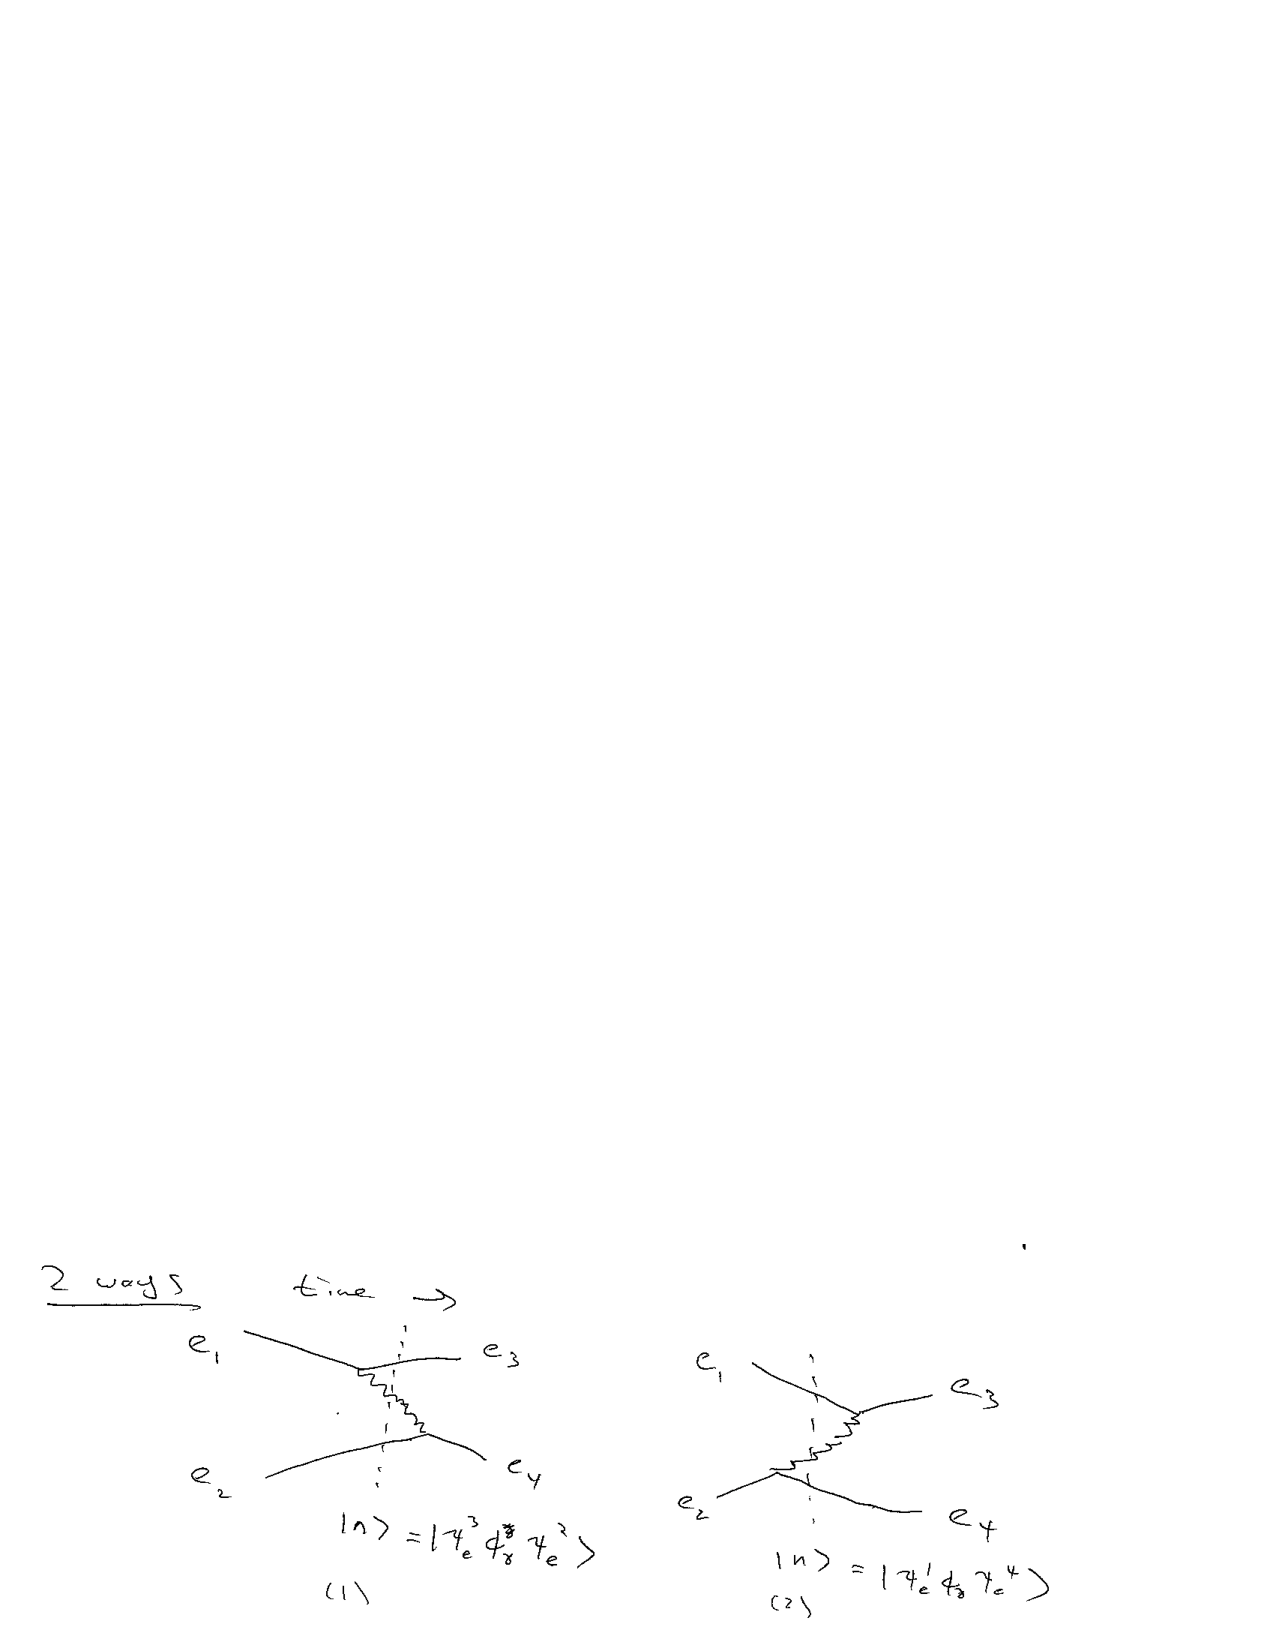
\includegraphics[width=0.99\textwidth]{./eeScattering.pdf}
\end{figure}





}
\end{document}

